\documentclass[a4paper,12pt]{report}

\usepackage{alltt, fancyvrb, url}
\usepackage{graphicx}
\usepackage[utf8]{inputenc}
\usepackage{float}
\usepackage{hyperref}

% Questo commentalo se vuoi scrivere in inglese.
\usepackage[italian]{babel}
\usepackage[italian]{cleveref}

\title{Relazione\\``Isaccoop''}

\author{Marco Costantini\\Andrea Dotti\\Daniele Pancottini\\Giacomo Pierbattista\\Dilaver Shtini}
\date{\today}

\begin{document}
\maketitle

\tableofcontents

\chapter{Analisi}
Il software mira a realizzare un gioco roguelike liberamente ispirato a ``The Binding Of Isaac". Con ``roguelike" si intende un videogioco tipicamente caratterizzato dall'esplorazione di un dungeon attraverso livelli generati proceduralmente e morte permanente del personaggio giocante.

\section{Requisiti}

\subsection*{Requisiti funzionali obbligatori}
\begin{itemize}
    \item Il protagonista inizierà la partita in una stanza iniziale vuota.
    \\Il giocatore può:
        \begin{itemize}
            \item muoversi liberamente all'interno di ogni stanza e sparare ``sfere di energia''
            \item passare da una stanza all'altra, solo dopo aver sconfitto tutti i \textbf{nemici} che si trovano al suo interno, se presenti
            \item raccogliere monete e cuori (``\textbf{item}'') sparsi nelle varie stanze, se presenti
            \item acquisire una vita raccogliendo i cuori sparsi nelle stanze
            \item comprare potenziamenti (\textbf{powerup}) nell'apposito negozio (\textbf{shop room}), usando le monete raccolte precedentemente
            \item raccogliere un powerup gratis nella stanza \textbf{treasure room}
            \item perdere una vita ogni volta che viene colpito da un nemico o da un proiettile lanciato da esso
            \item visualizzare la struttura del livello giocato nella \textbf{minimappa} per sapere in quale stanza si trova e vedere quali sono state completate
            \item visualizzare le sue (\textbf{``statistiche/caratteristiche"}), ad esempio: il numero di vite rimaste (indicate dai cuori), di monete raccolte, quanto danno riesce a infliggere ai nemici...
            \item il gioco finisce (game over) se il giocatore perde tutte le sue vite/cuori o quando sconfigge tutti i nemici in tutte le stanze, compreso il boss finale
        \end{itemize}

    \item Nel gioco vi sono cinque tipi di stanze:
        \begin{itemize}
            \item \textbf{START}: stanza iniziale vuota in cui il giocatore si trova all'inizio della partita
            \item \textbf{TREASURE}: stanza in cui si trova un powerup gratuito, che il giocatore può raccogliere per sconfiggere più facilmente i nemici
            \item \textbf{SHOP}: stanza in cui il giocatore può spendere le monete raccolte precedentemente per comprare altri powerup
            \item \textbf{STANDARD}: stanza in cui si trovano dei nemici e da cui il giocatore può uscire solo dopo averli sconfitti tutti
            \item \textbf{BOSS}: stanza in cui si trova il boss finale; una volta sconfitto, la partita termina.
        \end{itemize}
    \item Una semplice AI (Artificial Intelligence) gestirà i movimenti e gli attacchi dei nemici e del boss finale, i quali cercheranno di colpire il giocatore. Per AI si intende un semplice software che gestisce il movimento e il comportamento dei nemici.
    \item Implementazione della guida/tutorial al gioco, visualizzabile nel menu di gioco prima di iniziare una partita
    \item Gestione della pausa durante il gioco
\end{itemize}

\subsection*{Requisiti funzionali opzionali}
\begin{itemize}
    \item gestione di più livelli, ognuno indipendente dagli altri, con stanze differenti e difficoltà incrementali
    \item gestione del salvataggio a chiusura dell'applicazione per continuare la partita successivamente
    \item effetti sonori
    \item impostazioni di gioco (esempi a titolo indicativo e non esaustivo): \begin{itemize}
        \item scelta del numero minimo e massimo delle stanze che possono formare un livello
        \item numero di livelli da giocare in una partita
    \end{itemize} 
\end{itemize}

\subsection*{Requisiti non funzionali}
\begin{itemize}
    \item il software deve essere portabile, quindi deve essere eseguibile su macchine che eseguono Windows, Mac OS X e Linux/UNIX.
    \item Il software deve garantire un'esperienza di gioco adeguata (fluida, gradevole), indipendentemente dallo stato della partita.
\end{itemize}

\newpage
\section{Analisi e modello del dominio}
Il software permetterà al giocatore di avviare una sessione di gioco, che gestirà l'avanzamento del personaggio principale attraverso le varie stanze che formano il mondo di gioco (\textbf{``livello/level''}).
In un livello sono presenti un numero semicasuale di stanze; in alcune di esse saranno presenti i ``nemici'' da sconfiggere e gli ``item'', mentre in altre si potranno comprare/raccogliere i ``powerup''.
Una volta entrato in una stanza in cui si trovano i nemici, il giocatore dovrà sconfiggerli tutti per poter passare ad un altra.
I nemici saranno gestiti da una semplice AI (come descritto precedentemente) e cercheranno di attaccare e uccidere il giocatore. 
Per sconfiggere tali nemici, il giocatore spara le ``sfere di energia''. Utilizzando i powerup raccolti o comprati nello shop, il giocatore può sconfiggere più facilmente i nemici. 
Il giocatore perde una vita (indicate con i cuori/``hearts'') ogni volta che viene colpito da un nemico o da un proiettile sparato da esso.
Il gioco terminerà se il giocatore perde tutte le vite.

Le challenge principali di questo progetto sono:
\begin{itemize}
    \item gestione delle collisioni tra protagonista, item, powerup, nemici e muri delle stanze
    \item creazione dinamica delle stanze e con dei nemici al loro interno
\end{itemize}

\begin{figure}[H]
\centering{}
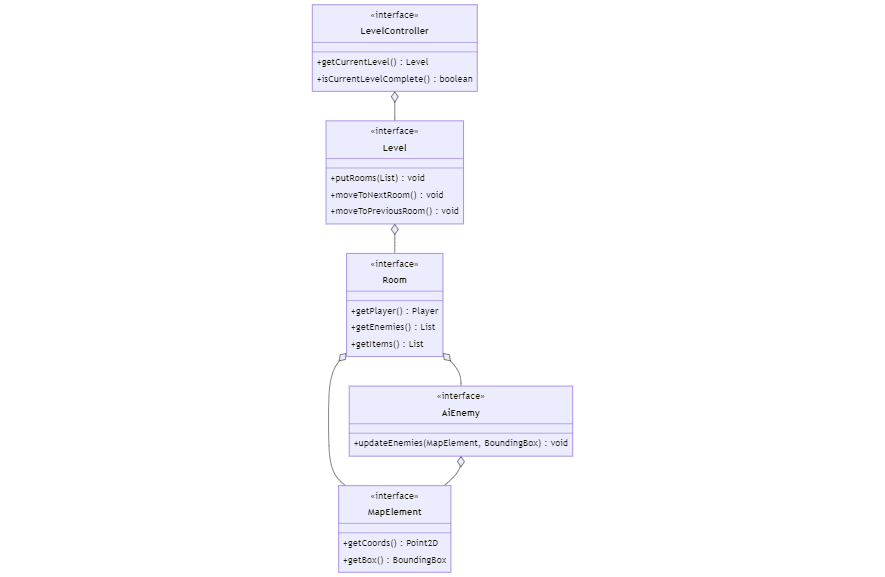
\includegraphics{img/analysis.pdf}
\caption{Schema UML dell'analisi del problema, con rappresentate le entità principali ed i rapporti fra loro}
\label{img:analysis}
\end{figure}


\chapter{Design}
\section{Architettura}
Nella progettazione, si è scelto di adottare il pattern architetturale MVC.
\begin{itemize}
	\item \textbf{Model}: ?
	\item \textbf{Controller}:
	 GameEngine?
	\item \textbf{View}:
	GameScene e Graphics.?
\end{itemize}

L'utilizzo di MVC consente di cambiare la tecnologia alla base della View senza modificare né Model né Controller del software: infatti sarà necessario cambiare l'implementazione dei file {TODO quali?} utilizzando la nuova tecnologia, sostituendo così l'implementazione attuale basata sul framework Swing con la nuova tecnologia scelta.


\begin{figure}[h]
\centering{}
\includegraphics[width=\textwidth]{img/arch}
\caption{Schema UML architetturale di GLaDOS. L'interfaccia \texttt{GLaDOS} è il controller del sistema, mentre \texttt{Input} ed \texttt{Output} sono le interfacce che mappano la view (o, più correttamente in questo specifico esempio, il boundary). Un'eventuale interfaccia grafica interattiva dovrà implementarle entrambe.}
\label{img:goodarch}
\end{figure}


In \Cref{img:goodarch} è esemplificato il diagramma UML architetturale.


\section{Design dettagliato}

\subsection*{Marco Costantini}
{TODO}

\subsection*{Andrea Dotti}
{TODO}
\subsection*{Daniele Pancottini}
{TODO}
\subsection*{Giacomo Pierbattista}
{TODO}
Nello sviluppo di Isaccoop mi sono occupato della creazione della mappa di gioco, costituita da un numero random di stanze,

\subsection*{Dilaver Shtini}
{TODO}

\subsection*{Esempio minimale (e quindi parziale) di sezione di progetto con UML ben realizzati}

\subsubsection{Personalità intercambiabili}

\begin{figure}[H]
\centering{}
\includegraphics[width=\textwidth]{img/strategy}
\caption{Rappresentazione UML del pattern Strategy per la personalità di GLaDOS}
\label{img:strategy}
\end{figure}

\paragraph{Problema} GLaDOS ha più personalità intercambiabili, la cui presenza deve essere trasparente al client.

\paragraph{Soluzione} Il sistema per la gestione della personalità utilizza il \textit{pattern Strategy}, come da
\Cref{img:strategy}: le implementazioni di \texttt{Personality} possono essere modificate, e la
modifica impatta direttamente sul comportamento di GLaDOS.

\subsubsection{Riuso del codice delle personalità}

\begin{figure}[H]
\centering{}
\includegraphics[width=\textwidth]{img/template}
\caption{Rappresentazione UML dell'applicazione del pattern Template Method alla gerarchia delle Personalità}
\label{img:template}
\end{figure}

\paragraph{Problema} In fase di sviluppo, sono state sviluppate due personalità, una buona ed una cattiva.
Quella buona restituisce sempre una torta vera, mentre quella cattiva restituisce sempre la
promessa di una torta che verrà in realtà disattesa.
Ci si è accorti che diverse personalità condividevano molto del comportamento,
portando a classi molto simili e a duplicazione.

\paragraph{Soluzione} Dato che le due personalità differiscono solo per il comportamento da effettuarsi in caso di percorso completato con successo,
è stato utilizzato il \textit{pattern template method} per massimizzare il riuso, come da \Cref{img:template}.
Il metodo template è \texttt{onSuccess()}, che chiama un metodo astratto e protetto
\texttt{makeCake()}.

\subsubsection{Gestione di output multipli}

\begin{figure}[H]
\centering{}
\includegraphics[width=.7\textwidth]{img/observer}
\caption{Il pattern Observer è usato per consentire a GLaDOS di informare tutti i sistemi di output in ascolto}
\label{img:observer}
\end{figure}

\paragraph{Problema} Il sistema deve supportare output multipli. In particolare, si richiede che vi sia un logger che stampa a terminale o su file,
e un'interfaccia grafica che mostri una rappresentazione grafica del sistema.

\paragraph{Soluzione} Dato che i due sistemi di reporting utilizzano le medesime informazioni, si è deciso di raggrupparli dietro l'interfaccia \texttt{Output}.
A questo punto, le due possibilità erano quelle di far sì che \texttt{GLaDOS} potesse pilotarle entrambe.
Invece di fare un sistema in cui questi output sono obbligatori e connessi, si è deciso di usare maggior flessibilità (anche in vista di future estensioni)
e di adottare una comunicazione uno-a-molti fra \texttt{GLaDOS} ed i sistemi di output.
La scelta è quindi ricaduta sul \textit{pattern Observer}: \texttt{GLaDOS} è observable, e le istanze di \texttt{Output} sono observer.
%
Il suo utilizzo è esemplificato in \Cref{img:observer}




\begin{figure}[h]
\centering{}
\includegraphics[width=\textwidth]{img/badarch}
\caption{Schema UML mal fatto e con una pessima descrizione, che non aiuta a capire. Don't try this at home.}
\label{img:badarch}
\end{figure}


\chapter{Sviluppo}
\section{Testing automatizzato}
Sono state realizzate diverse classi di test automatizzato, utilizzando JUnit 5.
Non sono stati realizzati test automatici sulla GUI per mancanza di tempo.
I test sono stati realizzati secondo quanto segue:
\subsection*{Marco Costantini}
\begin{itemize}
    \item TestItem
\end{itemize}
\subsection*{Andrea Dotti}
\begin{itemize}
    \item TestShop
\end{itemize}
\subsection*{Daniele Pancottini}
\begin{itemize}
    \item TestEnemy
\end{itemize}
\subsection*{Giacomo Pierbattista}
Ognuno dei seguenti file contiene un test per ogni metodo delle rispettive interfacce, in modo da verificare
il corretto funzionamento di ogni singolo metodo.
\begin{itemize}
    \item LevelControllerTest
    \item LevelFactoryTest
    \item LevelTest
    \item RoomBuilderTest
    \item RoomFactoryTest
    \item RoomTest
\end{itemize}

\subsection*{Dilaver Shtini}
\begin{itemize}
    \item TestPlayer
\end{itemize}



\section{Metodologia di lavoro}
Il lavoro è stato diviso tra i componenti del gruppo all'inizio, in modo da permettere a tutti di 
lavorare indipendentemente dagli altri il più possibile.
E' stato necessario riunirsi per discutere sull'implementazione e/o sulla dichiarazione di interfacce e 
classi comuni.

Abbiamo utilizzato lo strumento di version control \textbf{Git} per poter sviluppare il software in modo più agevole.
\\Il branch principale è stato denominato \textit{master}.
Dal \textit{master}, sono stati creati vari branch, chiamati ``feature-featureName''; ognuno di essi identificava la feature che doveva essere implementata. 
La divisione delle feature tra i vari componenti del gruppo è stata tale da permettere a ognuno di lavorare nel proprio branch indipendentemente dagli altri.
\\Abbiamo lavorato in modo tale che tutte le modifiche venissero apportate nei vari branch ``feature-featureName''; solo dopo aver testato che tutto funzionasse correttamente, tali modifiche sono state unite sul branch \textit{master}.
\\In questo modo, il software contenuto nel branch \textit{master} funzionava sempre correttamente.

\subsection*{Marco Costantini}
\\In autonomia, ho sviluppato
\begin{itemize}
    \item \begin{verbatim}it.unibo.isaccoop.core.* \end{verbatim} esclusa la funzione di pausa in GameLoopImpl.java
    \item \begin{verbatim}it.unibo.isaccoop.model.item.* \end{verbatim}
    \item \begin{verbatim}it.unibo.isaccoop.model.powerup.* \end{verbatim}
\end{itemize}
Ho sviluppato: 
\begin{itemize}
    \item in collaborazione con Daniele Pancottini: \begin{verbatim}it.unibo.isaccoop.graphics.factory.* \end{verbatim}
    \item in collaborazione con Andrea Dotti \begin{verbatim}it.unibo.isaccoop.model.boundingBox.* \end{verbatim}
    \item in collaborazione con Daniele Pancottini e Andrea Dotti:  
    \begin{itemize}
        \item \begin{verbatim}it.unibo.isaccoop.model.creator.* \end{verbatim} 
        \item \begin{verbatim}it.unibo.isaccoop.model.collision.* \end{verbatim}
    \end{itemize}
\end{itemize} 

\subsection*{Andrea Dotti}
Mi sono concentrato principalmente dello spawn di nemici, powerup e item nelle varie stanze, ho gestito gli input
da tastiera del giocatore. Mi sono focalizzato anche sul controllo delle collisioni con i BoundingBox, che sono serviti
ai miei compagni nella CollisionCheck.
In autonomia ho sviluppato:
\begin{itemize}
    \item \begin{verbatim}Shop.java e ShopImpl.java \end{verbatim}
    \item \begin{verbatim}it.unibo.isaccoop.input.* \end{verbatim}
    \item \begin{verbatim}it.unibo.isaccoop.model.spawn.* \end{verbatim}
\end{itemize}
Ho sviluppato: 
\begin{itemize}
\item in collaborazione con Marco Costantini \begin{verbatim}it.unibo.isaccoop.model.boundingBox.* \end{verbatim}
\item in collaborazione con Marco Costantini e Daniele Pancottini:
    \begin{itemize}
        \item \begin{verbatim}it.unibo.isaccoop.model.collision.* \end{verbatim}
        \item \begin{verbatim}it.unibo.isaccoop.model.creator.* \end{verbatim}
    \end{itemize}
\end{itemize}

\subsection*{Daniele Pancottini}
Ho sviluppato:
\begin{itemize}
    \item in collaborazione con Marco Costantini \begin{verbatim}it.unibo.isaccoop.graphics.factory.* \end{verbatim}
    \item in collaborazione con Dilaver Shtini 
    \begin{itemize}
        \item \begin{verbatim}it.unibo.isaccoop.model.action.* \end{verbatim}
        \item \begin{verbatim}it.unibo.isaccoop.model.ai.* \end{verbatim}
        \item \begin{verbatim}it.unibo.isaccoop.model.enemy.* \end{verbatim}
        \item \begin{verbatim}it.unibo.isaccoop.model.weapon.* \end{verbatim}
    \end{itemize}
    \item in collaborazione con Marco Costantini e Andrea Dotti
        \begin{itemize}
            \item \begin{verbatim}it.unibo.isaccoop.model.collision.* \end{verbatim}
            \item \begin{verbatim}it.unibo.isaccoop.model.creator.* \end{verbatim}
        \end{itemize}
    \item la funzione di pausa in GameLoopImpl.java
\end{itemize}

\subsection*{Giacomo Pierbattista}
Mi sono concentrato principalmente sulla progettazione del mondo di gioco (Level) e delle stanze (Room).
In autonomia, nel model, ho sviluppato le classi contenute nel package 
\begin{verbatim}it.unibo.isaccoop.model.room.* \end{verbatim} escludendo
\begin{verbatim}Shop.java e ShopImpl.java, \end{verbatim}
che implementano quanto segue:
\begin{itemize}
    \item creazione dinamica della mappa di gioco/livello, costituita da stanze
    \item passaggio del giocatore da una stanza all'altra
    \item minimappa.
\end{itemize}
e le enum Direction.java e RoomType.java.
\\Nella view ho sviluppato quanto segue:
\begin{itemize}
    \item guida utente (HelpGUI.java)
    \item pannello contenente la minimappa e le statistiche del giocatore (OverlayGUI.java)
    \item AbstractGUIFrame.java, GUIFrame.java
\end{itemize}

\subsection*{Dilaver Shtini}
In autonomia ho sviluppato:
\begin{itemize}
    \item \begin{verbatim}GameMenu.java \end{verbatim}
    \item \begin{verbatim}it.unibo.isaccoop.model.player.* \end{verbatim}
\end{itemize}
In collaborazione con Daniele Pancottini ho sviluppato:
    \begin{itemize}
        \item \begin{verbatim}it.unibo.isaccoop.model.action.* \end{verbatim}
        \item \begin{verbatim}it.unibo.isaccoop.model.ai.* \end{verbatim}
        \item \begin{verbatim}it.unibo.isaccoop.model.enemy.* \end{verbatim}
        \item \begin{verbatim}it.unibo.isaccoop.model.weapon.* \end{verbatim}
    \end{itemize}

\subsection*{In collaborazione}
\begin{itemize}
    \item \begin{verbatim}SwingGraphics.java\end{verbatim} e i file rimanenti riguardanti la view
    \item \begin{verbatim}it.unibo.isaccoop.model.common \end{verbatim}
\end{itemize}

\section{Note di sviluppo}
Abbiamo iniziato lo sviluppo a partire dalla repository \url{https://github.com/unibo-oop/sample-gradle-project}, compreso il \textbf{Gradle wrapper} fornito, per poter eseguire la build del progetto.
\subsection*{Marco Costantini}
{TODO}

\subsection*{Andrea Dotti}
{TODO}

\subsection*{Daniele Pancottini}
{TODO}

\subsection*{Giacomo Pierbattista}
Nello sviluppo ho utilizzato
\begin{itemize}
    \item \textbf{Optional} in molti file; alcuni esempi
    \begin{itemize}
        \item in RoomBuilder: \url{https://github.com/jackprb/OOP22-isaccoop/blob/master/src/main/java/it/unibo/isaccoop/model/room/RoomBuilder.java#L34}
        \item in RoomImpl: \url{https://github.com/jackprb/OOP22-isaccoop/blob/master/src/main/java/it/unibo/isaccoop/model/room/RoomImpl.java#L28}
    \end{itemize}
    \item \textbf{Stream} in molti file, ad esempio in LevelControllerImpl e nei file in cui sono state utilizzate liste e mappe
    \item \textbf{Lambda} insieme agli stream, in vari file, ad esempio in RoomImpl
    \item \textbf{Wildcard} in Roombuilder Utils ({TODO} spiega brevemente perché)
\end{itemize}
Per poter caricare il file contenente la guida utente dal filesystem, ho utilizzato \textbf{ClassLoader} in HelpGui.java; ho guardato qui 
\\\url{https://github.com/unibo-oop/example-with-get-resources/blob/master/src/main/java/it/unibo/getresource/UseGetResource.java#L35}.
\\Per ridimensionare un Jframe a seconda della risoluzione dello schermo in AbstractGUIFrame.java ho guardato qui: 
\\\url{https://github.com/unibo-oop/lab08/blob/solutions/83-mvc-io/src/main/java/it/unibo/mvc/SimpleGUI.java#L83} (linee 83-102).

\subsection*{Dilaver Shtini}
{TODO}



\chapter{Commenti finali}

\section{Autovalutazione e lavori futuri}
\subsection*{Marco Costantini}
{TODO}

\subsection*{Andrea Dotti}
{TODO}

\subsection*{Daniele Pancottini}
{TODO}

\subsection*{Giacomo Pierbattista}
{TODO}

\subsection*{Dilaver Shtini}
{TODO}


\section{Difficoltà incontrate e commenti per i docenti}
\subsection*{Marco Costantini}
{TODO}

\subsection*{Andrea Dotti}
{TODO}

\subsection*{Daniele Pancottini}
{TODO}

\subsection*{Giacomo Pierbattista}
{TODO}

\subsection*{Dilaver Shtini}
{TODO}


\appendix
\chapter{Guida utente}

\section*{Menu principale}
All'avvio dell'applicativo, l'utente si ritroverà nel menu di gioco, in cui troverà tre pulsanti:
\begin{itemize}
    \item \textbf{Play} per avviare la partita
    \item \textbf{Help} per visualizzare la guida utente 
    \item \textbf{Quit} per chiudere il gioco.
\end{itemize}
\\{FOTO MENU GIOCO}

\section*{Modalità di gioco}
\subsection*{Comandi del giocatore}
Esattamente come nel gioco ``The Binding of Isaac'', a cui questo applicativo si ispira liberamente, i comandi riguardanti il giocatore sono i seguenti:
\begin{itemize}
    \item \textbf{W}: Movimento verso l'alto
    \item \textbf{A}: Movimento verso sinistra
    \item \textbf{S}: Movimento verso il basso
    \item \textbf{D}: movimento verso destra
\end{itemize}
Il giocatore, per sconfiggere nemici, spara le ``onde di energia''
\begin{itemize}
    \item \textbf{↑} (Freccia SU): verso l'alto
    \item \textbf{↓} (Freccia GIU): verso il basso
    \item \textbf{←} (Freccia SINISTRA): verso sinistra
    \item \textbf{→} (Freccia DESTRA): verso destra
\end{itemize}

\subsection*{Altri comandi}
\begin{itemize}
    \item \textbf{Esc}: mette il gioco in pausa
    \item \textbf{P}: il giocatore si sposta nella stanza successiva
    \item \textbf{N}: il giocatore si sposta nella stanza precedente
\end{itemize}

\subsection*{Schermata di gioco}
Dopo aver cliccato il pulsante ``Play'' nel menu principale, l'utente visualizzerà la seguente schermata, caratterizzata da due sezioni principali:
\\{FOTO SCHERMATA DI GIOCO 1 STANZA}

\begin{itemize}
    \item \textbf{la stanza di gioco}, in alto, dove si muovono il giocatore e i nemici
    \item \textbf{la barra di stato}, in basso, dove vengono mostrate, da sinistra verso destra:
    \begin{itemize}
        \item \textit{minimappa}: mostra la struttura del livello, il numero di stanze che lo compongono e se tali stanze sono complete oppure no
        (una stanza è completa se non sono rimasti altri nemici da sconfiggere)
        \item \textit{statistiche del giocatore}: mostra alcune informazioni sullo stato del giocatore
        \item \textit{legenda}: spiega il significato dei colori utilizzati nella minimappa
    \end{itemize}
\end{itemize}

Se il giocatore viene colpito dai nemici e perde tutte le vite, la partita terminerà, mostrando la seguente schermata di game over.
{FOTO SCHERMATA DI GIOCO GAME OVER}

Quando il giocatore completa tutte le stanze, compresa quella del boss finale, comparirà la seguente schermata
{FOTO SCHERMATA DI GIOCO GAME COMPLETED}

Sia nel caso di game over, sia nel caso di vittoria, per tornare al menu principale, è sufficiente cliccare ovunque sopra la mappa di gioco.


\chapter{Esercitazioni di laboratorio}

\section*{Esempio}

\subsection{paperon.depaperoni@studio.unibo.it}

\begin{itemize}
 \item Laboratorio 04: \url{https://virtuale.unibo.it/mod/forum/discuss.php?d=12345#p123456}
 \item Laboratorio 05: \url{https://virtuale.unibo.it/mod/forum/discuss.php?d=22222#p222222}
 \item Laboratorio 06: \url{https://virtuale.unibo.it/mod/forum/discuss.php?d=99999#p999999}
 \item Laboratorio 07: \url{https://virtuale.unibo.it/mod/forum/discuss.php?d=22222#p222222}
 \item Laboratorio 08: \url{https://virtuale.unibo.it/mod/forum/discuss.php?d=99999#p999999}
 \item Laboratorio 09: \url{https://virtuale.unibo.it/mod/forum/discuss.php?d=22222#p222222}
 \item Laboratorio 10: \url{https://virtuale.unibo.it/mod/forum/discuss.php?d=99999#p999999}
 \item Laboratorio 11: \url{https://virtuale.unibo.it/mod/forum/discuss.php?d=22222#p222222}
\end{itemize}


\bibliographystyle{alpha}
\bibliography{13-template}
\begin{itemize}
    \item Nella fase di analisi abbiamo preso spunto dalla repository del prof. Alessandro Ricci. 
    \url{https://github.com/pslab-unibo/oop-game-prog-patterns-2022} 
\end{itemize}
\end{document}}